%%% PGCON 2013, Hackers Meeting
%%%
%%% The future of PostgreSQL Extensibility

\documentclass[english]{beamer}
\usepackage[utf8]{inputenc}
%%\usepackage[latin9]{inputenc}
\usepackage[T1]{fontenc}
\usepackage{babel}
\usepackage{eurosym}

\usepackage{minted}

\usepackage{beamerthemesplit}
%% \usetheme{Warsaw}
%% \usetheme{Frankfurt}
\usetheme{Boadilla}
\beamertemplatetransparentcovered

\title{PostgreSQL Extensibility}
\subtitle{is still doing baby steps}
\author{Dimitri Fontaine \newline\tiny{\texttt{dimitri@2ndQuadrant.fr}}}
\date{22 May 2013}
\logo{
\includegraphics[height=0.4cm]{2ndQuadrant-cross.png}}

\begin{document}

\frame{\titlepage}

\begin{frame}[fragile]
  \frametitle{Dimitri Fontaine}

  \begin{center}
    \textbf{PostgreSQL Extensibility}
    \vfill
    is a step towards the all mighty \textit{PostgreSQL Database Kernel}
  \end{center}
  \vfill

\begin{columns}[c]
\column{.75\textwidth} 

  \begin{itemize}
   \item<1-> \texttt{\textbf{CREATE EXTENSION}}
   \item<1-> \texttt{\textbf{CREATE EVENT TRIGGER}}
   \item<2-> \textit{EXTENSION TEMPLATES}
   \item<3-> \textit{DDL Execution Plans}
   \item<4-> \textit{In-catalogs binary objects}
   \item<4-> or at least \textit{bytecode}
  \end{itemize}  

\column{.25\textwidth}
\begin{center}
  
\includegraphics[height=5em]{distribution.jpg}
\end{center}
\end{columns}
\end{frame}

\begin{frame}[fragile]
  \frametitle{I know you don't want this in core:}

\begin{minted}{postgresql}
prompt=> CREATE EXTENSION pgxn;
CREATE EXTENSION

prompt=> CREATE EXTENSION awesome;
NOTICE: extension "awesome" is not locally available
NOTICE: updating repository pgxn
NOTICE: updating repository heroku
NOTICE: updating repository 2nQXN
NOTICE: found extension awesome, version 1.2, at heroku
NOTICE: fetching http://pgxn.org/awesome/awesome--1.2.sql
CREATE EXTENSION
\end{minted}
\end{frame}

\begin{frame}[fragile]
  \frametitle{What about this then?}

\begin{minted}{postgresql}
CREATE FUNCTION foo()
        RETURNS whatever
       LANGUAGE 'PL/C'
AS $$
   void support_function()
   {
       <some C code here>;
   }
   
   whatever *
   foo()
   {
           int c;
           
           <some C code here>;
   }
$$;
\end{minted}
\end{frame}

\frame{
  \frametitle{Let's talk about this...}

\begin{center}
  \textbf{Moar extensibility}
  \linebreak

  Also known as the only way to stop me proposing crazy ideas within huge
  patches to the \textit{core} product and team.
  \vfill

  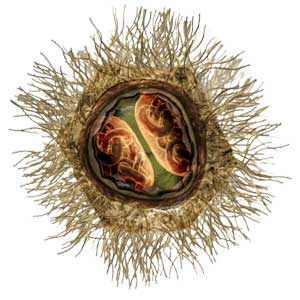
\includegraphics[height=9em]{in-core-replication.jpg}
\end{center}
}

\end{document}

\frame{\titlepage}
